\documentclass{article}\usepackage[]{graphicx}\usepackage[]{color}
% maxwidth is the original width if it is less than linewidth
% otherwise use linewidth (to make sure the graphics do not exceed the margin)
\makeatletter
\def\maxwidth{ %
  \ifdim\Gin@nat@width>\linewidth
    \linewidth
  \else
    \Gin@nat@width
  \fi
}
\makeatother

\definecolor{fgcolor}{rgb}{0.345, 0.345, 0.345}
\newcommand{\hlnum}[1]{\textcolor[rgb]{0.686,0.059,0.569}{#1}}%
\newcommand{\hlstr}[1]{\textcolor[rgb]{0.192,0.494,0.8}{#1}}%
\newcommand{\hlcom}[1]{\textcolor[rgb]{0.678,0.584,0.686}{\textit{#1}}}%
\newcommand{\hlopt}[1]{\textcolor[rgb]{0,0,0}{#1}}%
\newcommand{\hlstd}[1]{\textcolor[rgb]{0.345,0.345,0.345}{#1}}%
\newcommand{\hlkwa}[1]{\textcolor[rgb]{0.161,0.373,0.58}{\textbf{#1}}}%
\newcommand{\hlkwb}[1]{\textcolor[rgb]{0.69,0.353,0.396}{#1}}%
\newcommand{\hlkwc}[1]{\textcolor[rgb]{0.333,0.667,0.333}{#1}}%
\newcommand{\hlkwd}[1]{\textcolor[rgb]{0.737,0.353,0.396}{\textbf{#1}}}%
\let\hlipl\hlkwb

\usepackage{framed}
\makeatletter
\newenvironment{kframe}{%
 \def\at@end@of@kframe{}%
 \ifinner\ifhmode%
  \def\at@end@of@kframe{\end{minipage}}%
  \begin{minipage}{\columnwidth}%
 \fi\fi%
 \def\FrameCommand##1{\hskip\@totalleftmargin \hskip-\fboxsep
 \colorbox{shadecolor}{##1}\hskip-\fboxsep
     % There is no \\@totalrightmargin, so:
     \hskip-\linewidth \hskip-\@totalleftmargin \hskip\columnwidth}%
 \MakeFramed {\advance\hsize-\width
   \@totalleftmargin\z@ \linewidth\hsize
   \@setminipage}}%
 {\par\unskip\endMakeFramed%
 \at@end@of@kframe}
\makeatother

\definecolor{shadecolor}{rgb}{.97, .97, .97}
\definecolor{messagecolor}{rgb}{0, 0, 0}
\definecolor{warningcolor}{rgb}{1, 0, 1}
\definecolor{errorcolor}{rgb}{1, 0, 0}
\newenvironment{knitrout}{}{} % an empty environment to be redefined in TeX

\usepackage{alltt}
\usepackage{rotating}
\usepackage{graphicx, color, framed, alltt}
\usepackage{fullpage}
\usepackage{pdflscape}
\usepackage{placeins}
\usepackage{longtable}
\IfFileExists{upquote.sty}{\usepackage{upquote}}{}
\begin{document}



\section*{Analaysis of Public Housing in County Census Tracts and \\Proximity to CE(s)}

\textbf{Original Analysis}\\
\textbf{By: D. White}\\
\textbf{Date: 2019-11-13}\\
\\
----------------------------\\
\break
KNITR File: Report\textunderscore Logistic\textunderscore Model.Rnw \\
\begin{knitrout}
\definecolor{shadecolor}{rgb}{0.969, 0.969, 0.969}\color{fgcolor}\begin{kframe}
\begin{verbatim}
## [1] "Generated on: 2020-04-23 16:49:58"
\end{verbatim}
\end{kframe}
\end{knitrout}
  





Methods: A multi-step data processing routine was performed for each county to integrate spatial and tabular data sets. Census tract data were spatially joined with CEs, Section-8 voucher housing units, and Low-Income Housing Tax Credit (LIHTC) units. 
\\

Processing Steps:\\
HUD Housing Data\\
1. Section-8 Voucher Data downloaded and aggregated from HUD website for each county (2000-2008)(see Assisted\textunderscore Housing\textunderscore Data.csv)\\
Section-8 Voucher data are spatially located by census tract. Primary data attributes included a census tract "CODE", "YEAR", "NUMBER\textunderscore REPORTED", and others. Census tract data were a multi-year report for each census tract in the county (2000, 2004, and 2008). Each county was saved as a separate CSV file (COUNTY\textunderscore ABREV\textunderscore HUD.CSV).  \\
2. LIHTC Data downloaded and aggregated from HUD website for each county (2000-2008) (The Low-Income Housing Tax Credit Affordable housing data.csv) LIHTC data are spatially located by address. Primary data attributes included a census tract "HUD ID Number", "Year", "Project Name", "Project Address", "Total Low-Income Units", "Total Number of Units", and others.
Data files were modified for GIS processing (attribute labels cleaned up, shortned, characters removed, etc.) and added to a GIS.\\
LIHTC data were geocoded using the "ArcGIS World Geocoding Service". A total of 238 nationwide LIHTC addresses were geocoded. Except for two locations, 236 addresses were positively matched. A separate analysis was performed on the two other locations that were ties. The locations were verified and a final shapefile was created. Using the Select by Attribute tool in ArcGIS, each county was exported as a separate shapefile (County\textunderscore Tax\textunderscore Credit.shp) from the naitonwide data set.\\

County Census Tracts:\\
County census tract data were downloaded from the IPUMS/NHGIS (IPUMS.org) for each county from the 2000 Census (see folder "nghis0045\textunderscore csv"). A data merge was performed in R using the spatial package (sp:::merge) between Section-8 CSV file and the Census Tract Shapefile for each county to generate a aggregated working file using a common census tract code as unique identifier ("GISJoin"). The resulting file in R that was filtered for the maximum available year that was 2008 for each county (Figure 1).\\


HUD-Aggregated Tables:\\
Section-8 and LIHTC were aggregated into a common spatial data set. The geocoded LIHTC county shapefile was imported into R and duplicate check was run to remove potential replicate LIHTC HUD IDs. Data were aggregated to the final observed year for each county, unlike Section-8, LIHTC data were summed across time to reflect the final year of available LIHTC units for each county. Section-8 and LIHTC were combined using a spatial join (sf:::st\textunderscore join) in R. The resulting spatial file realized census tract data with a total number of Section-8 housing units and multiple observations of LIHTC units per census tract. Thus, a final data set needed to collapse reported LIHTC into a single observation for each census tract. Further processing generated "clean" unique Section-8 and LIHTC summed by county census tract (Figure 2 and 3, repspectively). \\

The data processing by county can be found in the path below.\\ 
C:\textbackslash Users\textbackslash whitedl\textbackslash Documents\textbackslash R\textunderscore Code\textbackslash HUD\textunderscore Project\textunderscore Code\textbackslash CNTYNAME\textunderscore Public\textunderscore Housing\textunderscore CE.R\\


Results\\
Descriptive Statistics:\\
Total census tracts per county are presented in Figure 1. With the exception of SAC, all counties had fewer than 100 census tracts. Douglas county had the group minimum of 8. Sacramento had a group maximum of 279. Explanatory variables had high zero counts with respect to prescence per census tract (Figure 4 and 5). Both groups show a large number of zeros, but LIHTC units were generally found in fewer census tracts. Section 8 units were more abundant than LIHTC units (Figures 6 and 7). However, LIHTC appear to have a higher density in census tracts (Figure 8). Sacramento had the largest total number of Section 8 and LIHTC units. Douglas county had the fewest Section 8 units and zero LIHTC units.\\  


Model:\\
A poisson logistic regression was performed on an all county data set to test the probability of a CE located in census tract dependent upon HUD housing counts (Tables 1-4). Table 5 presents the results of a zero-inflation model, however, an overdispersion test indicates that overdispersion was not present in the GLM-Poisson model (Table 4), and geneally not an issue for the county models. Tables 6-36 show results of the logistic-poisson model for each individual county. ALB and DGL were included in the county global model, but were not run as discrete county models due to small sample sizes. \\

Parameter coefficient estimates for the global model (all counties) (CE presence/abscence = LIHTC + Sec 8) were significant (Table 1). A positive coefficent will indicate that an increase in public housing is associated with an increase in the probability of a CE in a given Census Tract. A negative coefficent will imply that increased numbers of public housing units are associated with a decreased probability of a CE in a census tract. Section 8 units had a signficant negative effect (-0.007)(P$<$.01) and LIHTC units had a signficant positive effect (0.002)(P$<$.05). A significant negative constant was reported (-0.738)(P$<$.01). Overdispersion was not indicted (Table 4).\\

Sacramento and York had significant coefficient estimates for Section 8 and LIHTC units. For Sacramento, Section 8 units had a signficant negative effect (-0.016)(P$<$.05) and LIHTC units had a signficant postitive effect (0.003)(P$<$.01). A significant negative constant was reported (-1.970)(P$<$.01) (Table 30). Overdispersion was not indicted (Table 33). For York county,  Section 8 units had a signficant negative effect (-0.016)(P$<$.05) and LIHTC units had a signficant postitive effect (0.010)(P$<$.1) (Table 42). A significant negative constant was reported (-0.401)(P$<$.1). Overdispersion was not indicted (Table 44). For all other counties parameter coefficients were found to not be significant.

\pagebreak
\newpage
\FloatBarrier


\begin{knitrout}
\definecolor{shadecolor}{rgb}{0.969, 0.969, 0.969}\color{fgcolor}\begin{figure}
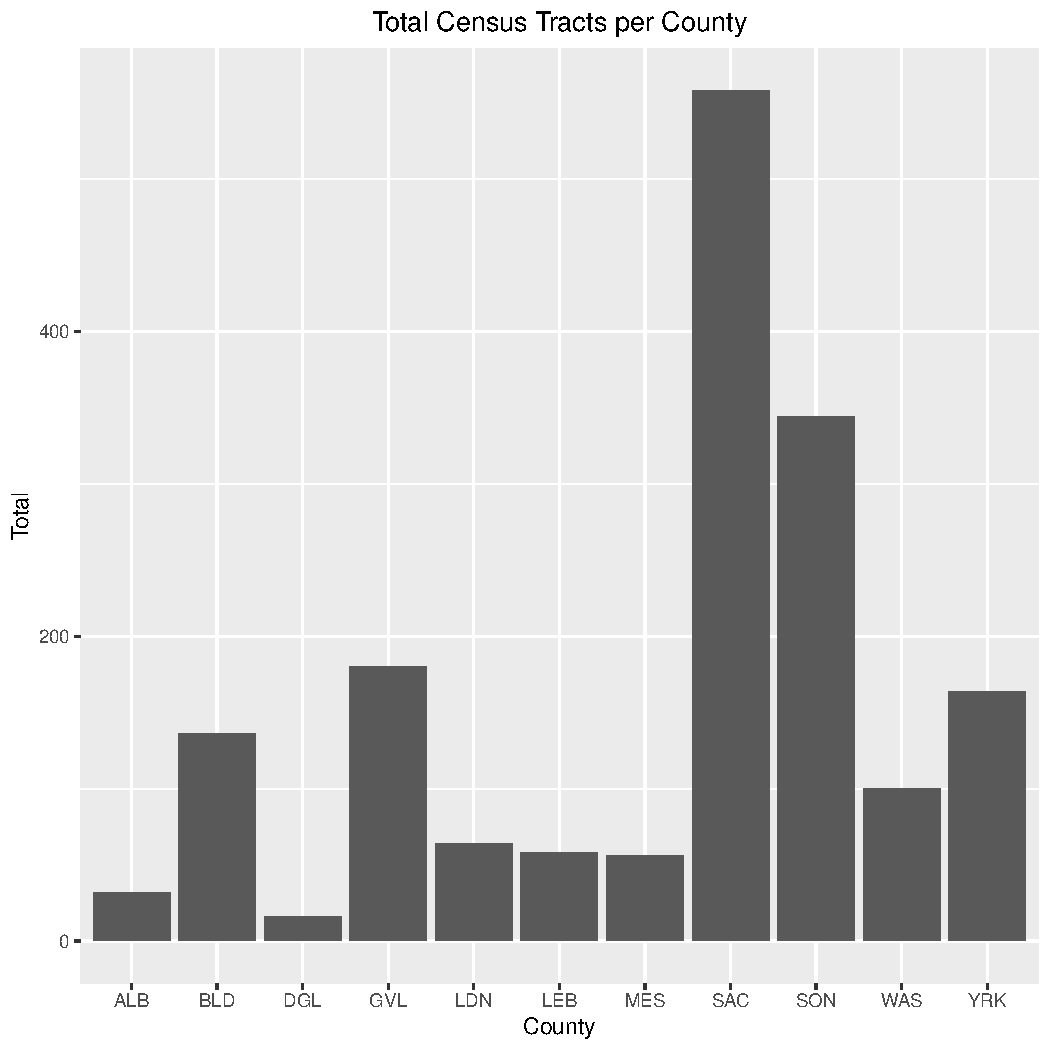
\includegraphics[width=\maxwidth]{figure/Bar_All_Counties_Tract-1} \caption[Total Census Tracts by County]{Total Census Tracts by County}\label{fig:Bar_All_Counties_Tract}
\end{figure}


\end{knitrout}

\pagebreak
\newpage
\FloatBarrier

\begin{knitrout}
\definecolor{shadecolor}{rgb}{0.969, 0.969, 0.969}\color{fgcolor}\begin{figure}
\includegraphics[width=1.1\linewidth]{C:/Users/whitedl/Box Sync/Default Sync Folder/Projects/NSF_CNH/HUD_Analysis/FinalFigures_Out/bldsec8} \caption[Section 8 Vouchers by Census Tract in Boulder, CO with CE Overlay]{Section 8 Vouchers by Census Tract in Boulder, CO with CE Overlay}\label{fig:Example_County_Census_Sec8}
\end{figure}


\end{knitrout}

\begin{knitrout}
\definecolor{shadecolor}{rgb}{0.969, 0.969, 0.969}\color{fgcolor}\begin{figure}
\includegraphics[width=1.1\linewidth]{C:/Users/whitedl/Box Sync/Default Sync Folder/Projects/NSF_CNH/HUD_Analysis/FinalFigures_Out/bldlihtc} \caption[LIHTC by Census Tract in Boulder, CO with CE Overlay]{LIHTC by Census Tract in Boulder, CO with CE Overlay}\label{fig:Example_County_Census_LITHC}
\end{figure}


\end{knitrout}
 
\pagebreak
\newpage
\FloatBarrier 
 
\begin{knitrout}
\definecolor{shadecolor}{rgb}{0.969, 0.969, 0.969}\color{fgcolor}\begin{figure}
\includegraphics[width=0.9\linewidth]{figure/Hist_All_Sec_8_Counties_Tract-1} \caption[Histogram of Section 8 Units]{Histogram of Section 8 Units}\label{fig:Hist_All_Sec_8_Counties_Tract}
\end{figure}


\end{knitrout}


\begin{knitrout}
\definecolor{shadecolor}{rgb}{0.969, 0.969, 0.969}\color{fgcolor}\begin{figure}
\includegraphics[width=\maxwidth]{figure/Hist_All_LIHTC_Counties_Tract-1} \caption[Histogram of LIHTC Units]{Histogram of LIHTC Units}\label{fig:Hist_All_LIHTC_Counties_Tract}
\end{figure}


\end{knitrout}


\begin{knitrout}
\definecolor{shadecolor}{rgb}{0.969, 0.969, 0.969}\color{fgcolor}\begin{figure}
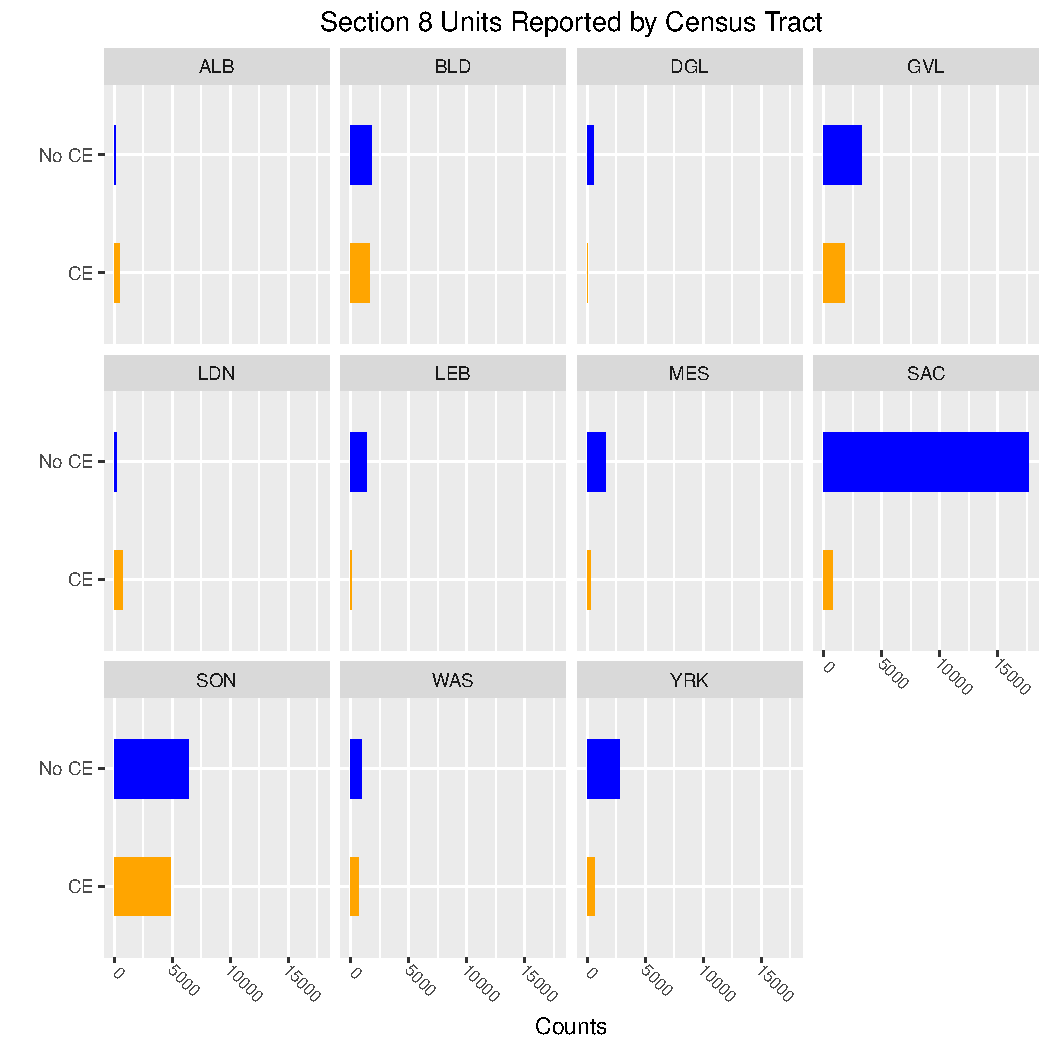
\includegraphics[width=\maxwidth]{figure/MultiPlot_SEC_8_Counts-1} \caption[Section 8 Units Reported by Census Tract]{Section 8 Units Reported by Census Tract}\label{fig:MultiPlot_SEC_8_Counts}
\end{figure}


\end{knitrout}


\begin{knitrout}
\definecolor{shadecolor}{rgb}{0.969, 0.969, 0.969}\color{fgcolor}\begin{figure}
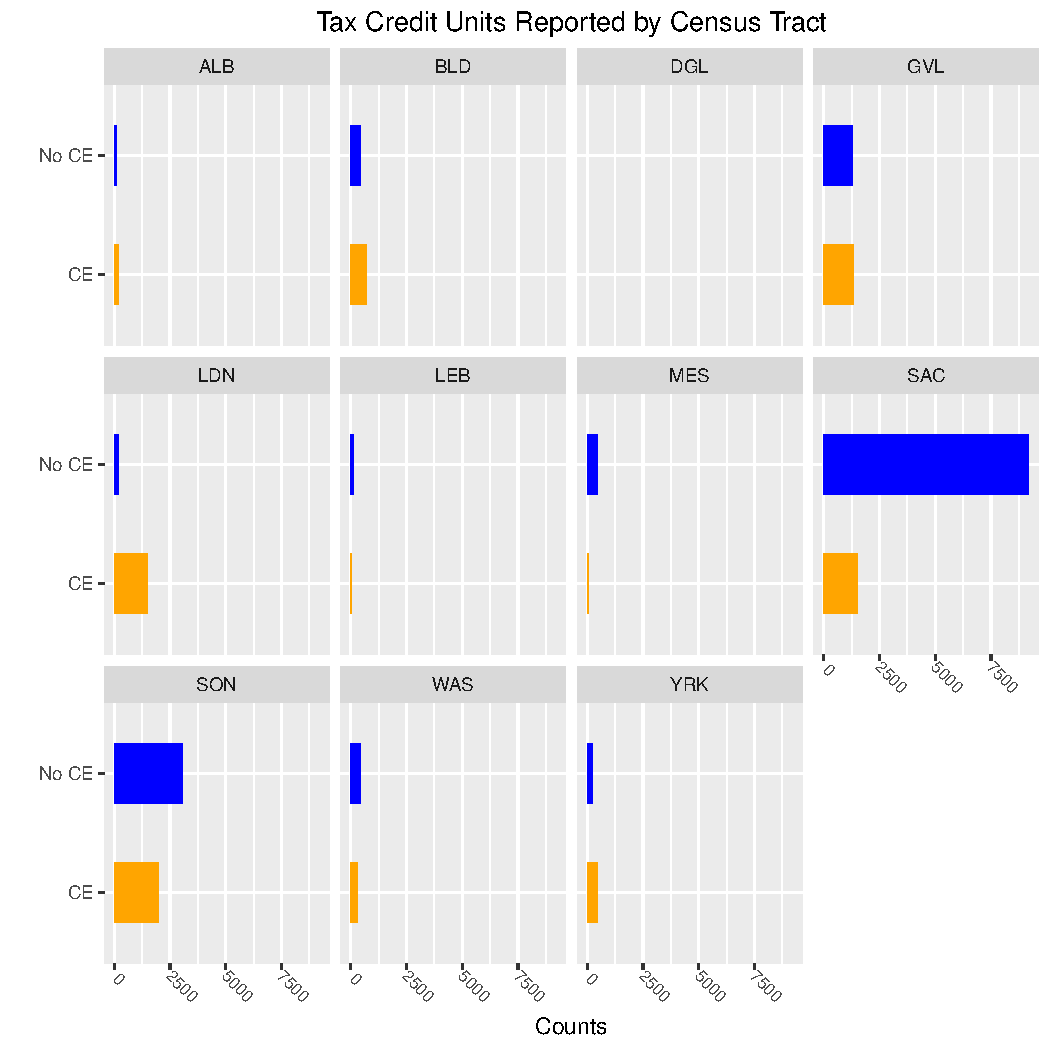
\includegraphics[width=\maxwidth]{figure/MultiPlot_Tax_Units_Counts-1} \caption[LIHTC Units Reported by Census Tract]{LIHTC Units Reported by Census Tract}\label{fig:MultiPlot_Tax_Units_Counts}
\end{figure}


\end{knitrout}


\begin{knitrout}
\definecolor{shadecolor}{rgb}{0.969, 0.969, 0.969}\color{fgcolor}\begin{figure}
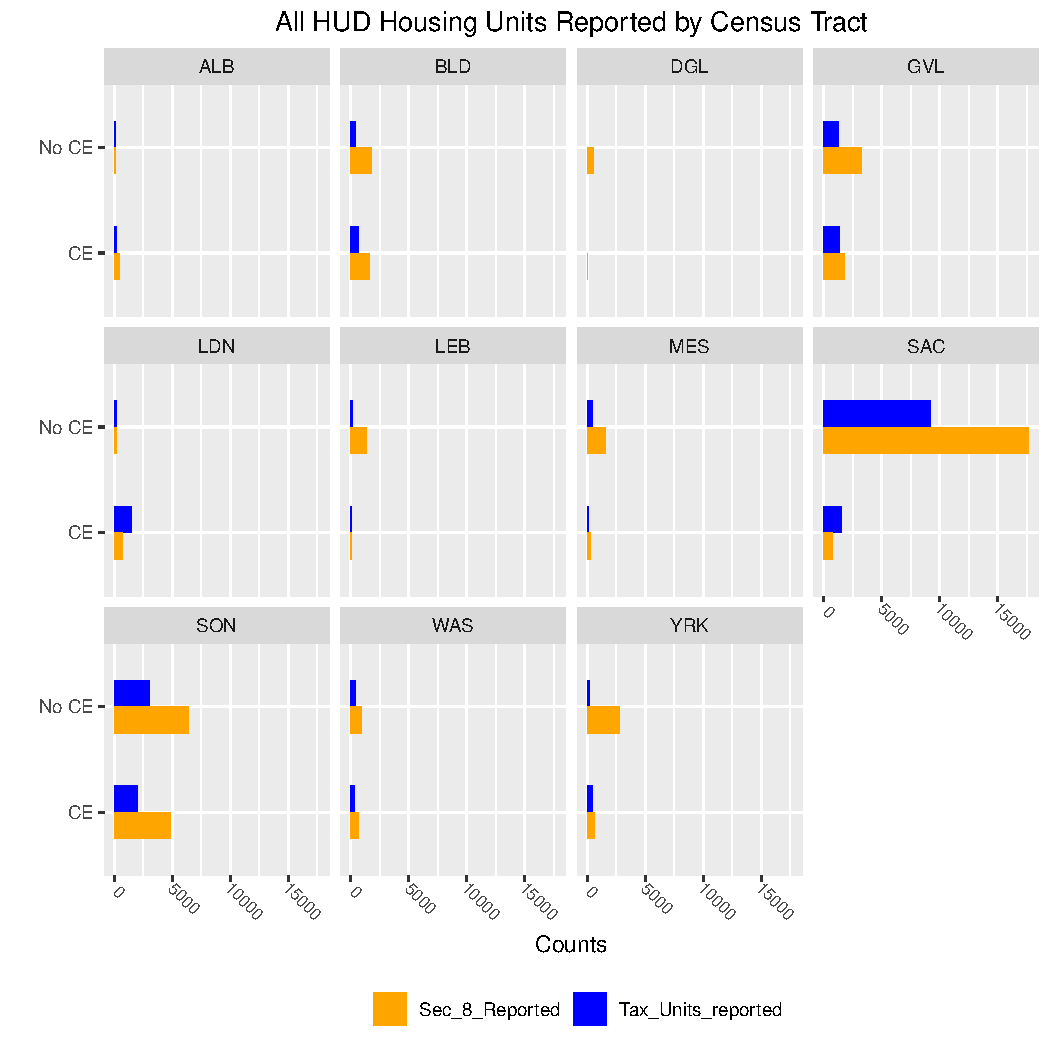
\includegraphics[width=\maxwidth]{figure/MultiPlot_All_Units_Counts_dodge-1} \caption[Housing Units Reported by Census Tract]{Housing Units Reported by Census Tract}\label{fig:MultiPlot_All_Units_Counts_dodge}
\end{figure}


\end{knitrout}


\begin{knitrout}
\definecolor{shadecolor}{rgb}{0.969, 0.969, 0.969}\color{fgcolor}\begin{figure}
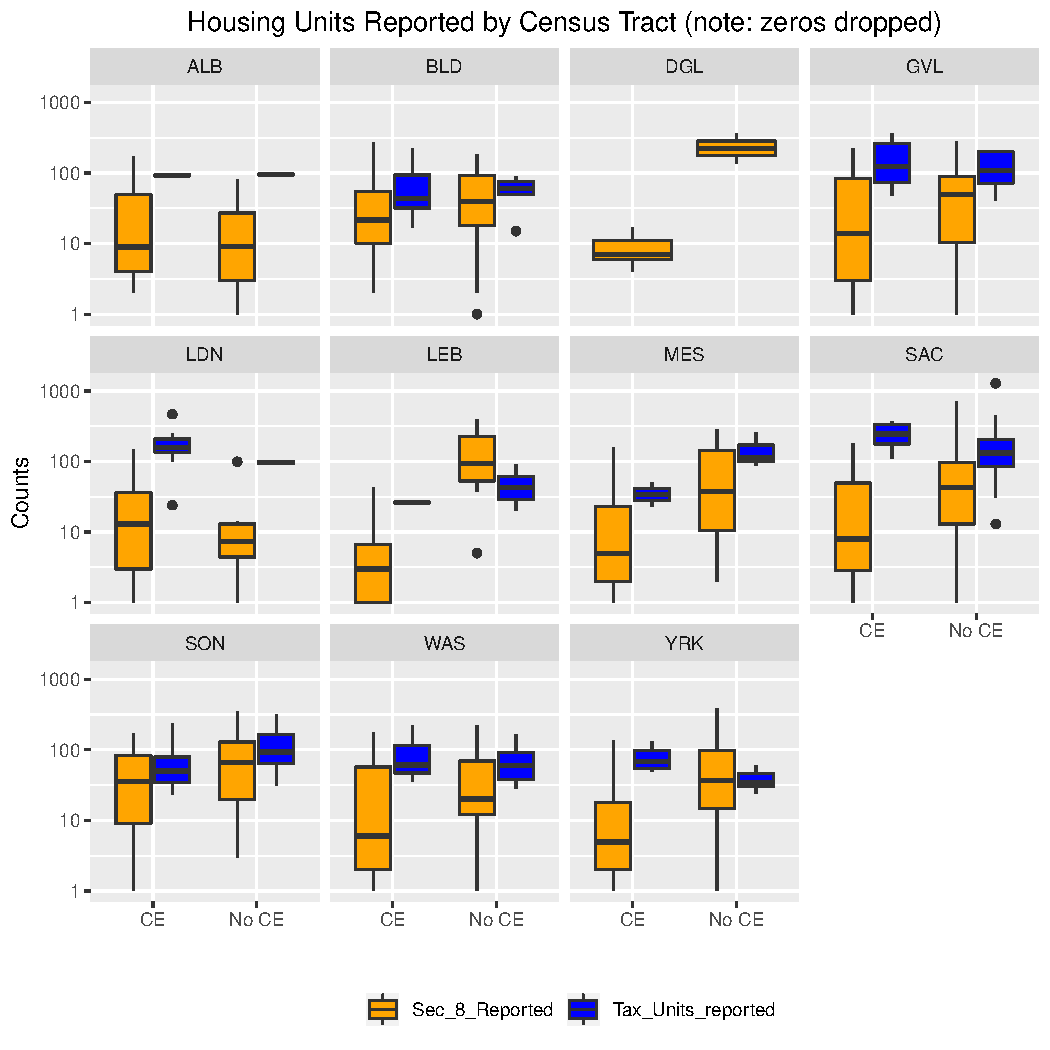
\includegraphics[width=\maxwidth]{figure/BoxPlot_All_Units-1} \caption[Housing Units Reported by Census Tract]{Housing Units Reported by Census Tract}\label{fig:BoxPlot_All_Units}
\end{figure}


\end{knitrout}

\pagebreak
\newpage
\FloatBarrier




% Table created by stargazer v.5.2.2 by Marek Hlavac, Harvard University. E-mail: hlavac at fas.harvard.edu
% Date and time: Thu, Apr 23, 2020 - 4:50:11 PM
% Requires LaTeX packages: dcolumn 
\begin{table}[!htbp] \centering 
  \caption{All Counties: Logistic Regression Results (GLM, Poisson) : HUD Housing} 
  \label{} 
\begin{tabular}{@{\extracolsep{5pt}}lD{.}{.}{-3} } 
\\[-1.8ex]\hline 
\hline \\[-1.8ex] 
 & \multicolumn{1}{c}{\textit{Dependent variable:}} \\ 
\cline{2-2} 
\\[-1.8ex] & \multicolumn{1}{c}{CE\_Present} \\ 
\hline \\[-1.8ex] 
 Sec\_8\_Reported & -0.007^{***} \\ 
  & (0.001) \\ 
  & \\ 
 Tax\_Units\_reported & 0.002^{**} \\ 
  & (0.001) \\ 
  & \\ 
 Constant & -0.738^{***} \\ 
  & (0.070) \\ 
  & \\ 
\hline \\[-1.8ex] 
Observations & \multicolumn{1}{c}{846} \\ 
Log Likelihood & \multicolumn{1}{c}{-594.702} \\ 
Akaike Inf. Crit. & \multicolumn{1}{c}{1,195.404} \\ 
\hline 
\hline \\[-1.8ex] 
\textit{Note:}  & \multicolumn{1}{r}{$^{*}$p$<$0.1; $^{**}$p$<$0.05; $^{***}$p$<$0.01} \\ 
\end{tabular} 
\end{table} 



% Table created by stargazer v.5.2.2 by Marek Hlavac, Harvard University. E-mail: hlavac at fas.harvard.edu
% Date and time: Thu, Apr 23, 2020 - 4:50:12 PM
% Requires LaTeX packages: dcolumn 
\begin{table}[!htbp] \centering 
  \caption{All Counties: Analysis of Deviance} 
  \label{} 
\begin{tabular}{@{\extracolsep{5pt}}lD{.}{.}{-3} D{.}{.}{-3} D{.}{.}{-3} D{.}{.}{-3} D{.}{.}{-3} D{.}{.}{-3} D{.}{.}{-3} } 
\\[-1.8ex]\hline 
\hline \\[-1.8ex] 
Statistic & \multicolumn{1}{c}{N} & \multicolumn{1}{c}{Mean} & \multicolumn{1}{c}{St. Dev.} & \multicolumn{1}{c}{Min} & \multicolumn{1}{c}{Pctl(25)} & \multicolumn{1}{c}{Pctl(75)} & \multicolumn{1}{c}{Max} \\ 
\hline \\[-1.8ex] 
Df & 2 & 1.000 & 0.000 & 1.000 & 1.000 & 1.000 & 1.000 \\ 
Deviance & 2 & 22.480 & 25.683 & 4.319 & 13.400 & 31.561 & 40.641 \\ 
Resid. Df & 3 & 844.000 & 1.000 & 843 & 843.5 & 844.5 & 845 \\ 
Resid. Dev & 3 & 593.830 & 24.805 & 577.404 & 579.563 & 602.043 & 622.364 \\ 
Pr(\textgreater Chi) & 2 & 0.019 & 0.027 & 0.000 & 0.009 & 0.028 & 0.038 \\ 
\hline \\[-1.8ex] 
\end{tabular} 
\end{table} 



% Table created by stargazer v.5.2.2 by Marek Hlavac, Harvard University. E-mail: hlavac at fas.harvard.edu
% Date and time: Thu, Apr 23, 2020 - 4:50:12 PM
% Requires LaTeX packages: dcolumn 
\begin{table}[!htbp] \centering 
  \caption{All Counties: McFadden Statistic:similar to R2} 
  \label{} 
\begin{tabular}{@{\extracolsep{5pt}} D{.}{.}{-3} D{.}{.}{-3} D{.}{.}{-3} D{.}{.}{-3} D{.}{.}{-3} D{.}{.}{-3} } 
\\[-1.8ex]\hline 
\hline \\[-1.8ex] 
\multicolumn{1}{c}{llh} & \multicolumn{1}{c}{llhNull} & \multicolumn{1}{c}{G2} & \multicolumn{1}{c}{McFadden} & \multicolumn{1}{c}{r2ML} & \multicolumn{1}{c}{r2CU} \\ 
\hline \\[-1.8ex] 
-594.702 & -617.182 & 44.960 & 0.036 & 0.052 & 0.067 \\ 
\hline \\[-1.8ex] 
\end{tabular} 
\end{table} 



% Table created by stargazer v.5.2.2 by Marek Hlavac, Harvard University. E-mail: hlavac at fas.harvard.edu
% Date and time: Thu, Apr 23, 2020 - 4:50:13 PM
% Requires LaTeX packages: dcolumn 
\begin{table}[!htbp] \centering 
  \caption{Overdisperson Test} 
  \label{} 
\begin{tabular}{@{\extracolsep{5pt}} D{.}{.}{-3} D{.}{.}{-3} D{.}{.}{-3} D{.}{.}{-3} D{.}{.}{-3} D{.}{.}{-3} D{.}{.}{-3} D{.}{.}{-3} } 
\\[-1.8ex]\hline 
\hline \\[-1.8ex] 
\multicolumn{1}{c}{} & \multicolumn{1}{c}{statistic} & \multicolumn{1}{c}{p.value} & \multicolumn{1}{c}{estimate} & \multicolumn{1}{c}{null.value} & \multicolumn{1}{c}{alternative} & \multicolumn{1}{c}{method} & \multicolumn{1}{c}{data.name} \\ 
\hline \\[-1.8ex] 
\multicolumn{1}{c}{z} & -11.262 & 1 & -0.362 & 0 & \multicolumn{1}{c}{greater} & \multicolumn{1}{c}{Overdispersion test} & \multicolumn{1}{c}{model1\_Poisson} \\ 
\hline \\[-1.8ex] 
\end{tabular} 
\end{table} 



\pagebreak
\newpage
\FloatBarrier



% Table created by stargazer v.5.2.2 by Marek Hlavac, Harvard University. E-mail: hlavac at fas.harvard.edu
% Date and time: Thu, Apr 23, 2020 - 4:50:14 PM
% Requires LaTeX packages: dcolumn 
\begin{table}[!htbp] \centering 
  \caption{All Counties: Logistic Regression Results, Zero Inflation Model (Poisson Distribution): HUD Housing} 
  \label{} 
\begin{tabular}{@{\extracolsep{5pt}}lD{.}{.}{-3} } 
\\[-1.8ex]\hline 
\hline \\[-1.8ex] 
 & \multicolumn{1}{c}{\textit{Dependent variable:}} \\ 
\cline{2-2} 
\\[-1.8ex] & \multicolumn{1}{c}{CE\_Present} \\ 
\hline \\[-1.8ex] 
 Sec\_8\_Reported & -0.008^{***} \\ 
  & (0.001) \\ 
  & \\ 
 Tax\_Units\_reported & 0.003^{***} \\ 
  & (0.001) \\ 
  & \\ 
 Constant & -0.745^{***} \\ 
  & (0.070) \\ 
  & \\ 
\hline \\[-1.8ex] 
Observations & \multicolumn{1}{c}{846} \\ 
Log Likelihood & \multicolumn{1}{c}{-592.625} \\ 
\hline 
\hline \\[-1.8ex] 
\textit{Note:}  & \multicolumn{1}{r}{$^{*}$p$<$0.1; $^{**}$p$<$0.05; $^{***}$p$<$0.01} \\ 
\end{tabular} 
\end{table} 



\pagebreak
\newpage
\FloatBarrier



% Table created by stargazer v.5.2.2 by Marek Hlavac, Harvard University. E-mail: hlavac at fas.harvard.edu
% Date and time: Thu, Apr 23, 2020 - 4:50:14 PM
% Requires LaTeX packages: dcolumn 
\begin{table}[!htbp] \centering 
  \caption{BLD Regression Results: HUD Housing} 
  \label{} 
\begin{tabular}{@{\extracolsep{5pt}}lD{.}{.}{-3} } 
\\[-1.8ex]\hline 
\hline \\[-1.8ex] 
 & \multicolumn{1}{c}{\textit{Dependent variable:}} \\ 
\cline{2-2} 
\\[-1.8ex] & \multicolumn{1}{c}{CE\_Present} \\ 
\hline \\[-1.8ex] 
 Sec\_8\_Reported & -0.005 \\ 
  & (0.004) \\ 
  & \\ 
 Tax\_Units\_reported & 0.005 \\ 
  & (0.005) \\ 
  & \\ 
 Constant & -0.478^{**} \\ 
  & (0.215) \\ 
  & \\ 
\hline \\[-1.8ex] 
Observations & \multicolumn{1}{c}{68} \\ 
Log Likelihood & \multicolumn{1}{c}{-58.659} \\ 
Akaike Inf. Crit. & \multicolumn{1}{c}{123.318} \\ 
\hline 
\hline \\[-1.8ex] 
\textit{Note:}  & \multicolumn{1}{r}{$^{*}$p$<$0.1; $^{**}$p$<$0.05; $^{***}$p$<$0.01} \\ 
\end{tabular} 
\end{table} 



% Table created by stargazer v.5.2.2 by Marek Hlavac, Harvard University. E-mail: hlavac at fas.harvard.edu
% Date and time: Thu, Apr 23, 2020 - 4:50:14 PM
% Requires LaTeX packages: dcolumn 
\begin{table}[!htbp] \centering 
  \caption{BLD: Analysis of Deviance} 
  \label{} 
\begin{tabular}{@{\extracolsep{5pt}}lD{.}{.}{-3} D{.}{.}{-3} D{.}{.}{-3} D{.}{.}{-3} D{.}{.}{-3} D{.}{.}{-3} D{.}{.}{-3} } 
\\[-1.8ex]\hline 
\hline \\[-1.8ex] 
Statistic & \multicolumn{1}{c}{N} & \multicolumn{1}{c}{Mean} & \multicolumn{1}{c}{St. Dev.} & \multicolumn{1}{c}{Min} & \multicolumn{1}{c}{Pctl(25)} & \multicolumn{1}{c}{Pctl(75)} & \multicolumn{1}{c}{Max} \\ 
\hline \\[-1.8ex] 
Df & 2 & 1.000 & 0.000 & 1.000 & 1.000 & 1.000 & 1.000 \\ 
Deviance & 2 & 0.859 & 0.250 & 0.682 & 0.770 & 0.947 & 1.036 \\ 
Resid. Df & 3 & 66.000 & 1.000 & 65 & 65.5 & 66.5 & 67 \\ 
Resid. Dev & 3 & 44.236 & 0.865 & 43.318 & 43.836 & 44.695 & 45.036 \\ 
Pr(\textgreater Chi) & 2 & 0.359 & 0.071 & 0.309 & 0.334 & 0.384 & 0.409 \\ 
\hline \\[-1.8ex] 
\end{tabular} 
\end{table} 



% Table created by stargazer v.5.2.2 by Marek Hlavac, Harvard University. E-mail: hlavac at fas.harvard.edu
% Date and time: Thu, Apr 23, 2020 - 4:50:14 PM
% Requires LaTeX packages: dcolumn 
\begin{table}[!htbp] \centering 
  \caption{BLD: McFadden Statistic:similar to R2} 
  \label{} 
\begin{tabular}{@{\extracolsep{5pt}} D{.}{.}{-3} D{.}{.}{-3} D{.}{.}{-3} D{.}{.}{-3} D{.}{.}{-3} D{.}{.}{-3} } 
\\[-1.8ex]\hline 
\hline \\[-1.8ex] 
\multicolumn{1}{c}{llh} & \multicolumn{1}{c}{llhNull} & \multicolumn{1}{c}{G2} & \multicolumn{1}{c}{McFadden} & \multicolumn{1}{c}{r2ML} & \multicolumn{1}{c}{r2CU} \\ 
\hline \\[-1.8ex] 
-58.659 & -59.518 & 1.718 & 0.014 & 0.025 & 0.030 \\ 
\hline \\[-1.8ex] 
\end{tabular} 
\end{table} 



% Table created by stargazer v.5.2.2 by Marek Hlavac, Harvard University. E-mail: hlavac at fas.harvard.edu
% Date and time: Thu, Apr 23, 2020 - 4:50:14 PM
% Requires LaTeX packages: dcolumn 
\begin{table}[!htbp] \centering 
  \caption{BLD Overdisperson Test} 
  \label{} 
\begin{tabular}{@{\extracolsep{5pt}} D{.}{.}{-3} D{.}{.}{-3} D{.}{.}{-3} D{.}{.}{-3} D{.}{.}{-3} D{.}{.}{-3} D{.}{.}{-3} D{.}{.}{-3} } 
\\[-1.8ex]\hline 
\hline \\[-1.8ex] 
\multicolumn{1}{c}{} & \multicolumn{1}{c}{statistic} & \multicolumn{1}{c}{p.value} & \multicolumn{1}{c}{estimate} & \multicolumn{1}{c}{null.value} & \multicolumn{1}{c}{alternative} & \multicolumn{1}{c}{method} & \multicolumn{1}{c}{data.name} \\ 
\hline \\[-1.8ex] 
\multicolumn{1}{c}{z} & -4.550 & 1.000 & -0.544 & 0 & \multicolumn{1}{c}{greater} & \multicolumn{1}{c}{Overdispersion test} & \multicolumn{1}{c}{BLD\_model1} \\ 
\hline \\[-1.8ex] 
\end{tabular} 
\end{table} 




% Table created by stargazer v.5.2.2 by Marek Hlavac, Harvard University. E-mail: hlavac at fas.harvard.edu
% Date and time: Thu, Apr 23, 2020 - 4:50:14 PM
% Requires LaTeX packages: dcolumn 
\begin{table}[!htbp] \centering 
  \caption{CHS Regression Results: HUD Housing} 
  \label{} 
\begin{tabular}{@{\extracolsep{5pt}}lD{.}{.}{-3} } 
\\[-1.8ex]\hline 
\hline \\[-1.8ex] 
 & \multicolumn{1}{c}{\textit{Dependent variable:}} \\ 
\cline{2-2} 
\\[-1.8ex] & \multicolumn{1}{c}{CE\_Present} \\ 
\hline \\[-1.8ex] 
 Sec\_8\_Reported & -0.005 \\ 
  & (0.004) \\ 
  & \\ 
 Tax\_Units\_reported & -0.005 \\ 
  & (0.011) \\ 
  & \\ 
 Constant & -0.931^{***} \\ 
  & (0.260) \\ 
  & \\ 
\hline \\[-1.8ex] 
Observations & \multicolumn{1}{c}{78} \\ 
Log Likelihood & \multicolumn{1}{c}{-45.890} \\ 
Akaike Inf. Crit. & \multicolumn{1}{c}{97.780} \\ 
\hline 
\hline \\[-1.8ex] 
\textit{Note:}  & \multicolumn{1}{r}{$^{*}$p$<$0.1; $^{**}$p$<$0.05; $^{***}$p$<$0.01} \\ 
\end{tabular} 
\end{table} 



% Table created by stargazer v.5.2.2 by Marek Hlavac, Harvard University. E-mail: hlavac at fas.harvard.edu
% Date and time: Thu, Apr 23, 2020 - 4:50:14 PM
% Requires LaTeX packages: dcolumn 
\begin{table}[!htbp] \centering 
  \caption{CHS: Analysis of Deviance} 
  \label{} 
\begin{tabular}{@{\extracolsep{5pt}}lD{.}{.}{-3} D{.}{.}{-3} D{.}{.}{-3} D{.}{.}{-3} D{.}{.}{-3} D{.}{.}{-3} D{.}{.}{-3} } 
\\[-1.8ex]\hline 
\hline \\[-1.8ex] 
Statistic & \multicolumn{1}{c}{N} & \multicolumn{1}{c}{Mean} & \multicolumn{1}{c}{St. Dev.} & \multicolumn{1}{c}{Min} & \multicolumn{1}{c}{Pctl(25)} & \multicolumn{1}{c}{Pctl(75)} & \multicolumn{1}{c}{Max} \\ 
\hline \\[-1.8ex] 
Df & 2 & 1.000 & 0.000 & 1.000 & 1.000 & 1.000 & 1.000 \\ 
Deviance & 2 & 2.666 & 3.512 & 0.183 & 1.424 & 3.907 & 5.149 \\ 
Resid. Df & 3 & 76.000 & 1.000 & 75 & 75.5 & 76.5 & 77 \\ 
Resid. Dev & 3 & 51.618 & 3.027 & 49.780 & 49.872 & 52.537 & 55.112 \\ 
Pr(\textgreater Chi) & 2 & 0.346 & 0.457 & 0.023 & 0.185 & 0.508 & 0.669 \\ 
\hline \\[-1.8ex] 
\end{tabular} 
\end{table} 



% Table created by stargazer v.5.2.2 by Marek Hlavac, Harvard University. E-mail: hlavac at fas.harvard.edu
% Date and time: Thu, Apr 23, 2020 - 4:50:14 PM
% Requires LaTeX packages: dcolumn 
\begin{table}[!htbp] \centering 
  \caption{CHS: McFadden Statistic:similar to R2} 
  \label{} 
\begin{tabular}{@{\extracolsep{5pt}} D{.}{.}{-3} D{.}{.}{-3} D{.}{.}{-3} D{.}{.}{-3} D{.}{.}{-3} D{.}{.}{-3} } 
\\[-1.8ex]\hline 
\hline \\[-1.8ex] 
\multicolumn{1}{c}{llh} & \multicolumn{1}{c}{llhNull} & \multicolumn{1}{c}{G2} & \multicolumn{1}{c}{McFadden} & \multicolumn{1}{c}{r2ML} & \multicolumn{1}{c}{r2CU} \\ 
\hline \\[-1.8ex] 
-45.890 & -48.556 & 5.332 & 0.055 & 0.066 & 0.093 \\ 
\hline \\[-1.8ex] 
\end{tabular} 
\end{table} 



% Table created by stargazer v.5.2.2 by Marek Hlavac, Harvard University. E-mail: hlavac at fas.harvard.edu
% Date and time: Thu, Apr 23, 2020 - 4:50:14 PM
% Requires LaTeX packages: dcolumn 
\begin{table}[!htbp] \centering 
  \caption{CHS Overdisperson Test} 
  \label{} 
\begin{tabular}{@{\extracolsep{5pt}} D{.}{.}{-3} D{.}{.}{-3} D{.}{.}{-3} D{.}{.}{-3} D{.}{.}{-3} D{.}{.}{-3} D{.}{.}{-3} D{.}{.}{-3} } 
\\[-1.8ex]\hline 
\hline \\[-1.8ex] 
\multicolumn{1}{c}{} & \multicolumn{1}{c}{statistic} & \multicolumn{1}{c}{p.value} & \multicolumn{1}{c}{estimate} & \multicolumn{1}{c}{null.value} & \multicolumn{1}{c}{alternative} & \multicolumn{1}{c}{method} & \multicolumn{1}{c}{data.name} \\ 
\hline \\[-1.8ex] 
\multicolumn{1}{c}{z} & -2.778 & 0.997 & -0.269 & 0 & \multicolumn{1}{c}{greater} & \multicolumn{1}{c}{Overdispersion test} & \multicolumn{1}{c}{CHS\_model1} \\ 
\hline \\[-1.8ex] 
\end{tabular} 
\end{table} 



% Table created by stargazer v.5.2.2 by Marek Hlavac, Harvard University. E-mail: hlavac at fas.harvard.edu
% Date and time: Thu, Apr 23, 2020 - 4:50:14 PM
% Requires LaTeX packages: dcolumn 
\begin{table}[!htbp] \centering 
  \caption{GVL Regression Results: HUD Housing} 
  \label{} 
\begin{tabular}{@{\extracolsep{5pt}}lD{.}{.}{-3} } 
\\[-1.8ex]\hline 
\hline \\[-1.8ex] 
 & \multicolumn{1}{c}{\textit{Dependent variable:}} \\ 
\cline{2-2} 
\\[-1.8ex] & \multicolumn{1}{c}{CE\_Present} \\ 
\hline \\[-1.8ex] 
 Sec\_8\_Reported & -0.003 \\ 
  & (0.003) \\ 
  & \\ 
 Tax\_Units\_reported & 0.002 \\ 
  & (0.002) \\ 
  & \\ 
 Constant & -0.771^{***} \\ 
  & (0.203) \\ 
  & \\ 
\hline \\[-1.8ex] 
Observations & \multicolumn{1}{c}{90} \\ 
Log Likelihood & \multicolumn{1}{c}{-69.907} \\ 
Akaike Inf. Crit. & \multicolumn{1}{c}{145.814} \\ 
\hline 
\hline \\[-1.8ex] 
\textit{Note:}  & \multicolumn{1}{r}{$^{*}$p$<$0.1; $^{**}$p$<$0.05; $^{***}$p$<$0.01} \\ 
\end{tabular} 
\end{table} 



% Table created by stargazer v.5.2.2 by Marek Hlavac, Harvard University. E-mail: hlavac at fas.harvard.edu
% Date and time: Thu, Apr 23, 2020 - 4:50:14 PM
% Requires LaTeX packages: dcolumn 
\begin{table}[!htbp] \centering 
  \caption{GVL: Analysis of Deviance} 
  \label{} 
\begin{tabular}{@{\extracolsep{5pt}}lD{.}{.}{-3} D{.}{.}{-3} D{.}{.}{-3} D{.}{.}{-3} D{.}{.}{-3} D{.}{.}{-3} D{.}{.}{-3} } 
\\[-1.8ex]\hline 
\hline \\[-1.8ex] 
Statistic & \multicolumn{1}{c}{N} & \multicolumn{1}{c}{Mean} & \multicolumn{1}{c}{St. Dev.} & \multicolumn{1}{c}{Min} & \multicolumn{1}{c}{Pctl(25)} & \multicolumn{1}{c}{Pctl(75)} & \multicolumn{1}{c}{Max} \\ 
\hline \\[-1.8ex] 
Df & 2 & 1.000 & 0.000 & 1.000 & 1.000 & 1.000 & 1.000 \\ 
Deviance & 2 & 0.858 & 0.237 & 0.690 & 0.774 & 0.941 & 1.025 \\ 
Resid. Df & 3 & 88.000 & 1.000 & 87 & 87.5 & 88.5 & 89 \\ 
Resid. Dev & 3 & 64.727 & 0.863 & 63.814 & 64.326 & 65.184 & 65.529 \\ 
Pr(\textgreater Chi) & 2 & 0.359 & 0.067 & 0.311 & 0.335 & 0.382 & 0.406 \\ 
\hline \\[-1.8ex] 
\end{tabular} 
\end{table} 



% Table created by stargazer v.5.2.2 by Marek Hlavac, Harvard University. E-mail: hlavac at fas.harvard.edu
% Date and time: Thu, Apr 23, 2020 - 4:50:15 PM
% Requires LaTeX packages: dcolumn 
\begin{table}[!htbp] \centering 
  \caption{GVL: McFadden Statistic:similar to R2} 
  \label{} 
\begin{tabular}{@{\extracolsep{5pt}} D{.}{.}{-3} D{.}{.}{-3} D{.}{.}{-3} D{.}{.}{-3} D{.}{.}{-3} D{.}{.}{-3} } 
\\[-1.8ex]\hline 
\hline \\[-1.8ex] 
\multicolumn{1}{c}{llh} & \multicolumn{1}{c}{llhNull} & \multicolumn{1}{c}{G2} & \multicolumn{1}{c}{McFadden} & \multicolumn{1}{c}{r2ML} & \multicolumn{1}{c}{r2CU} \\ 
\hline \\[-1.8ex] 
-69.907 & -70.764 & 1.715 & 0.012 & 0.019 & 0.024 \\ 
\hline \\[-1.8ex] 
\end{tabular} 
\end{table} 



% Table created by stargazer v.5.2.2 by Marek Hlavac, Harvard University. E-mail: hlavac at fas.harvard.edu
% Date and time: Thu, Apr 23, 2020 - 4:50:15 PM
% Requires LaTeX packages: dcolumn 
\begin{table}[!htbp] \centering 
  \caption{GVL Overdisperson Test} 
  \label{} 
\begin{tabular}{@{\extracolsep{5pt}} D{.}{.}{-3} D{.}{.}{-3} D{.}{.}{-3} D{.}{.}{-3} D{.}{.}{-3} D{.}{.}{-3} D{.}{.}{-3} D{.}{.}{-3} } 
\\[-1.8ex]\hline 
\hline \\[-1.8ex] 
\multicolumn{1}{c}{} & \multicolumn{1}{c}{statistic} & \multicolumn{1}{c}{p.value} & \multicolumn{1}{c}{estimate} & \multicolumn{1}{c}{null.value} & \multicolumn{1}{c}{alternative} & \multicolumn{1}{c}{method} & \multicolumn{1}{c}{data.name} \\ 
\hline \\[-1.8ex] 
\multicolumn{1}{c}{z} & -4.091 & 1.000 & -0.422 & 0 & \multicolumn{1}{c}{greater} & \multicolumn{1}{c}{Overdispersion test} & \multicolumn{1}{c}{GVL\_model1} \\ 
\hline \\[-1.8ex] 
\end{tabular} 
\end{table} 





% Table created by stargazer v.5.2.2 by Marek Hlavac, Harvard University. E-mail: hlavac at fas.harvard.edu
% Date and time: Thu, Apr 23, 2020 - 4:50:15 PM
% Requires LaTeX packages: dcolumn 
\begin{table}[!htbp] \centering 
  \caption{LDN Regression Results: HUD Housing} 
  \label{} 
\begin{tabular}{@{\extracolsep{5pt}}lD{.}{.}{-3} } 
\\[-1.8ex]\hline 
\hline \\[-1.8ex] 
 & \multicolumn{1}{c}{\textit{Dependent variable:}} \\ 
\cline{2-2} 
\\[-1.8ex] & \multicolumn{1}{c}{CE\_Present} \\ 
\hline \\[-1.8ex] 
 Sec\_8\_Reported & 0.001 \\ 
  & (0.006) \\ 
  & \\ 
 Tax\_Units\_reported & 0.001 \\ 
  & (0.002) \\ 
  & \\ 
 Constant & -0.469^{*} \\ 
  & (0.266) \\ 
  & \\ 
\hline \\[-1.8ex] 
Observations & \multicolumn{1}{c}{32} \\ 
Log Likelihood & \multicolumn{1}{c}{-30.002} \\ 
Akaike Inf. Crit. & \multicolumn{1}{c}{66.004} \\ 
\hline 
\hline \\[-1.8ex] 
\textit{Note:}  & \multicolumn{1}{r}{$^{*}$p$<$0.1; $^{**}$p$<$0.05; $^{***}$p$<$0.01} \\ 
\end{tabular} 
\end{table} 



% Table created by stargazer v.5.2.2 by Marek Hlavac, Harvard University. E-mail: hlavac at fas.harvard.edu
% Date and time: Thu, Apr 23, 2020 - 4:50:15 PM
% Requires LaTeX packages: dcolumn 
\begin{table}[!htbp] \centering 
  \caption{LDN: Analysis of Deviance} 
  \label{} 
\begin{tabular}{@{\extracolsep{5pt}}lD{.}{.}{-3} D{.}{.}{-3} D{.}{.}{-3} D{.}{.}{-3} D{.}{.}{-3} D{.}{.}{-3} D{.}{.}{-3} } 
\\[-1.8ex]\hline 
\hline \\[-1.8ex] 
Statistic & \multicolumn{1}{c}{N} & \multicolumn{1}{c}{Mean} & \multicolumn{1}{c}{St. Dev.} & \multicolumn{1}{c}{Min} & \multicolumn{1}{c}{Pctl(25)} & \multicolumn{1}{c}{Pctl(75)} & \multicolumn{1}{c}{Max} \\ 
\hline \\[-1.8ex] 
Df & 2 & 1.000 & 0.000 & 1.000 & 1.000 & 1.000 & 1.000 \\ 
Deviance & 2 & 0.241 & 0.083 & 0.182 & 0.212 & 0.271 & 0.300 \\ 
Resid. Df & 3 & 30.000 & 1.000 & 29 & 29.5 & 30.5 & 31 \\ 
Resid. Dev & 3 & 16.225 & 0.244 & 16.004 & 16.095 & 16.336 & 16.487 \\ 
Pr(\textgreater Chi) & 2 & 0.626 & 0.061 & 0.584 & 0.605 & 0.648 & 0.669 \\ 
\hline \\[-1.8ex] 
\end{tabular} 
\end{table} 



% Table created by stargazer v.5.2.2 by Marek Hlavac, Harvard University. E-mail: hlavac at fas.harvard.edu
% Date and time: Thu, Apr 23, 2020 - 4:50:15 PM
% Requires LaTeX packages: dcolumn 
\begin{table}[!htbp] \centering 
  \caption{LDN: McFadden Statistic:similar to R2} 
  \label{} 
\begin{tabular}{@{\extracolsep{5pt}} D{.}{.}{-3} D{.}{.}{-3} D{.}{.}{-3} D{.}{.}{-3} D{.}{.}{-3} D{.}{.}{-3} } 
\\[-1.8ex]\hline 
\hline \\[-1.8ex] 
\multicolumn{1}{c}{llh} & \multicolumn{1}{c}{llhNull} & \multicolumn{1}{c}{G2} & \multicolumn{1}{c}{McFadden} & \multicolumn{1}{c}{r2ML} & \multicolumn{1}{c}{r2CU} \\ 
\hline \\[-1.8ex] 
-30.002 & -30.243 & 0.483 & 0.008 & 0.015 & 0.018 \\ 
\hline \\[-1.8ex] 
\end{tabular} 
\end{table} 



% Table created by stargazer v.5.2.2 by Marek Hlavac, Harvard University. E-mail: hlavac at fas.harvard.edu
% Date and time: Thu, Apr 23, 2020 - 4:50:15 PM
% Requires LaTeX packages: dcolumn 
\begin{table}[!htbp] \centering 
  \caption{LDN Overdisperson Test} 
  \label{} 
\begin{tabular}{@{\extracolsep{5pt}} D{.}{.}{-3} D{.}{.}{-3} D{.}{.}{-3} D{.}{.}{-3} D{.}{.}{-3} D{.}{.}{-3} D{.}{.}{-3} D{.}{.}{-3} } 
\\[-1.8ex]\hline 
\hline \\[-1.8ex] 
\multicolumn{1}{c}{} & \multicolumn{1}{c}{statistic} & \multicolumn{1}{c}{p.value} & \multicolumn{1}{c}{estimate} & \multicolumn{1}{c}{null.value} & \multicolumn{1}{c}{alternative} & \multicolumn{1}{c}{method} & \multicolumn{1}{c}{data.name} \\ 
\hline \\[-1.8ex] 
\multicolumn{1}{c}{z} & -4.213 & 1.000 & -0.687 & 0 & \multicolumn{1}{c}{greater} & \multicolumn{1}{c}{Overdispersion test} & \multicolumn{1}{c}{LDN\_model1} \\ 
\hline \\[-1.8ex] 
\end{tabular} 
\end{table} 




% Table created by stargazer v.5.2.2 by Marek Hlavac, Harvard University. E-mail: hlavac at fas.harvard.edu
% Date and time: Thu, Apr 23, 2020 - 4:50:15 PM
% Requires LaTeX packages: dcolumn 
\begin{table}[!htbp] \centering 
  \caption{LEB Regression Results: HUD Housing} 
  \label{} 
\begin{tabular}{@{\extracolsep{5pt}}lD{.}{.}{-3} } 
\\[-1.8ex]\hline 
\hline \\[-1.8ex] 
 & \multicolumn{1}{c}{\textit{Dependent variable:}} \\ 
\cline{2-2} 
\\[-1.8ex] & \multicolumn{1}{c}{CE\_Present} \\ 
\hline \\[-1.8ex] 
 Sec\_8\_Reported & -0.032 \\ 
  & (0.020) \\ 
  & \\ 
 Tax\_Units\_reported & 0.017 \\ 
  & (0.040) \\ 
  & \\ 
 Constant & 0.004 \\ 
  & (0.241) \\ 
  & \\ 
\hline \\[-1.8ex] 
Observations & \multicolumn{1}{c}{29} \\ 
Log Likelihood & \multicolumn{1}{c}{-22.141} \\ 
Akaike Inf. Crit. & \multicolumn{1}{c}{50.283} \\ 
\hline 
\hline \\[-1.8ex] 
\textit{Note:}  & \multicolumn{1}{r}{$^{*}$p$<$0.1; $^{**}$p$<$0.05; $^{***}$p$<$0.01} \\ 
\end{tabular} 
\end{table} 



% Table created by stargazer v.5.2.2 by Marek Hlavac, Harvard University. E-mail: hlavac at fas.harvard.edu
% Date and time: Thu, Apr 23, 2020 - 4:50:15 PM
% Requires LaTeX packages: dcolumn 
\begin{table}[!htbp] \centering 
  \caption{LEB: Analysis of Deviance} 
  \label{} 
\begin{tabular}{@{\extracolsep{5pt}}lD{.}{.}{-3} D{.}{.}{-3} D{.}{.}{-3} D{.}{.}{-3} D{.}{.}{-3} D{.}{.}{-3} D{.}{.}{-3} } 
\\[-1.8ex]\hline 
\hline \\[-1.8ex] 
Statistic & \multicolumn{1}{c}{N} & \multicolumn{1}{c}{Mean} & \multicolumn{1}{c}{St. Dev.} & \multicolumn{1}{c}{Min} & \multicolumn{1}{c}{Pctl(25)} & \multicolumn{1}{c}{Pctl(75)} & \multicolumn{1}{c}{Max} \\ 
\hline \\[-1.8ex] 
Df & 2 & 1.000 & 0.000 & 1.000 & 1.000 & 1.000 & 1.000 \\ 
Deviance & 2 & 5.290 & 7.260 & 0.156 & 2.723 & 7.857 & 10.424 \\ 
Resid. Df & 3 & 27.000 & 1.000 & 26 & 26.5 & 27.5 & 28 \\ 
Resid. Dev & 3 & 7.861 & 6.064 & 4.283 & 4.361 & 9.651 & 14.863 \\ 
Pr(\textgreater Chi) & 2 & 0.347 & 0.489 & 0.001 & 0.174 & 0.520 & 0.693 \\ 
\hline \\[-1.8ex] 
\end{tabular} 
\end{table} 



% Table created by stargazer v.5.2.2 by Marek Hlavac, Harvard University. E-mail: hlavac at fas.harvard.edu
% Date and time: Thu, Apr 23, 2020 - 4:50:15 PM
% Requires LaTeX packages: dcolumn 
\begin{table}[!htbp] \centering 
  \caption{LEB: McFadden Statistic:similar to R2} 
  \label{} 
\begin{tabular}{@{\extracolsep{5pt}} D{.}{.}{-3} D{.}{.}{-3} D{.}{.}{-3} D{.}{.}{-3} D{.}{.}{-3} D{.}{.}{-3} } 
\\[-1.8ex]\hline 
\hline \\[-1.8ex] 
\multicolumn{1}{c}{llh} & \multicolumn{1}{c}{llhNull} & \multicolumn{1}{c}{G2} & \multicolumn{1}{c}{McFadden} & \multicolumn{1}{c}{r2ML} & \multicolumn{1}{c}{r2CU} \\ 
\hline \\[-1.8ex] 
-22.141 & -27.431 & 10.580 & 0.193 & 0.306 & 0.360 \\ 
\hline \\[-1.8ex] 
\end{tabular} 
\end{table} 



% Table created by stargazer v.5.2.2 by Marek Hlavac, Harvard University. E-mail: hlavac at fas.harvard.edu
% Date and time: Thu, Apr 23, 2020 - 4:50:15 PM
% Requires LaTeX packages: dcolumn 
\begin{table}[!htbp] \centering 
  \caption{LEB Overdisperson Test} 
  \label{} 
\begin{tabular}{@{\extracolsep{5pt}} D{.}{.}{-3} D{.}{.}{-3} D{.}{.}{-3} D{.}{.}{-3} D{.}{.}{-3} D{.}{.}{-3} D{.}{.}{-3} D{.}{.}{-3} } 
\\[-1.8ex]\hline 
\hline \\[-1.8ex] 
\multicolumn{1}{c}{} & \multicolumn{1}{c}{statistic} & \multicolumn{1}{c}{p.value} & \multicolumn{1}{c}{estimate} & \multicolumn{1}{c}{null.value} & \multicolumn{1}{c}{alternative} & \multicolumn{1}{c}{method} & \multicolumn{1}{c}{data.name} \\ 
\hline \\[-1.8ex] 
\multicolumn{1}{c}{z} & -6.024 & 1 & -0.690 & 0 & \multicolumn{1}{c}{greater} & \multicolumn{1}{c}{Overdispersion test} & \multicolumn{1}{c}{LEB\_model1} \\ 
\hline \\[-1.8ex] 
\end{tabular} 
\end{table} 




% Table created by stargazer v.5.2.2 by Marek Hlavac, Harvard University. E-mail: hlavac at fas.harvard.edu
% Date and time: Thu, Apr 23, 2020 - 4:50:15 PM
% Requires LaTeX packages: dcolumn 
\begin{table}[!htbp] \centering 
  \caption{MES Regression Results: HUD Housing} 
  \label{} 
\begin{tabular}{@{\extracolsep{5pt}}lD{.}{.}{-3} } 
\\[-1.8ex]\hline 
\hline \\[-1.8ex] 
 & \multicolumn{1}{c}{\textit{Dependent variable:}} \\ 
\cline{2-2} 
\\[-1.8ex] & \multicolumn{1}{c}{CE\_Present} \\ 
\hline \\[-1.8ex] 
 Sec\_8\_Reported & -0.009 \\ 
  & (0.009) \\ 
  & \\ 
 Tax\_Units\_reported & 0.003 \\ 
  & (0.014) \\ 
  & \\ 
 Constant & -0.657^{*} \\ 
  & (0.373) \\ 
  & \\ 
\hline \\[-1.8ex] 
Observations & \multicolumn{1}{c}{28} \\ 
Log Likelihood & \multicolumn{1}{c}{-19.084} \\ 
Akaike Inf. Crit. & \multicolumn{1}{c}{44.168} \\ 
\hline 
\hline \\[-1.8ex] 
\textit{Note:}  & \multicolumn{1}{r}{$^{*}$p$<$0.1; $^{**}$p$<$0.05; $^{***}$p$<$0.01} \\ 
\end{tabular} 
\end{table} 



% Table created by stargazer v.5.2.2 by Marek Hlavac, Harvard University. E-mail: hlavac at fas.harvard.edu
% Date and time: Thu, Apr 23, 2020 - 4:50:15 PM
% Requires LaTeX packages: dcolumn 
\begin{table}[!htbp] \centering 
  \caption{MES: Analysis of Deviance} 
  \label{} 
\begin{tabular}{@{\extracolsep{5pt}}lD{.}{.}{-3} D{.}{.}{-3} D{.}{.}{-3} D{.}{.}{-3} D{.}{.}{-3} D{.}{.}{-3} D{.}{.}{-3} } 
\\[-1.8ex]\hline 
\hline \\[-1.8ex] 
Statistic & \multicolumn{1}{c}{N} & \multicolumn{1}{c}{Mean} & \multicolumn{1}{c}{St. Dev.} & \multicolumn{1}{c}{Min} & \multicolumn{1}{c}{Pctl(25)} & \multicolumn{1}{c}{Pctl(75)} & \multicolumn{1}{c}{Max} \\ 
\hline \\[-1.8ex] 
Df & 2 & 1.000 & 0.000 & 1.000 & 1.000 & 1.000 & 1.000 \\ 
Deviance & 2 & 1.212 & 1.647 & 0.047 & 0.630 & 1.795 & 2.377 \\ 
Resid. Df & 3 & 26.000 & 1.000 & 25 & 25.5 & 26.5 & 27 \\ 
Resid. Dev & 3 & 18.992 & 1.386 & 18.168 & 18.192 & 19.404 & 20.592 \\ 
Pr(\textgreater Chi) & 2 & 0.475 & 0.498 & 0.123 & 0.299 & 0.652 & 0.828 \\ 
\hline \\[-1.8ex] 
\end{tabular} 
\end{table} 



% Table created by stargazer v.5.2.2 by Marek Hlavac, Harvard University. E-mail: hlavac at fas.harvard.edu
% Date and time: Thu, Apr 23, 2020 - 4:50:15 PM
% Requires LaTeX packages: dcolumn 
\begin{table}[!htbp] \centering 
  \caption{MES: McFadden Statistic:similar to R2} 
  \label{} 
\begin{tabular}{@{\extracolsep{5pt}} D{.}{.}{-3} D{.}{.}{-3} D{.}{.}{-3} D{.}{.}{-3} D{.}{.}{-3} D{.}{.}{-3} } 
\\[-1.8ex]\hline 
\hline \\[-1.8ex] 
\multicolumn{1}{c}{llh} & \multicolumn{1}{c}{llhNull} & \multicolumn{1}{c}{G2} & \multicolumn{1}{c}{McFadden} & \multicolumn{1}{c}{r2ML} & \multicolumn{1}{c}{r2CU} \\ 
\hline \\[-1.8ex] 
-19.084 & -20.296 & 2.424 & 0.060 & 0.083 & 0.108 \\ 
\hline \\[-1.8ex] 
\end{tabular} 
\end{table} 



% Table created by stargazer v.5.2.2 by Marek Hlavac, Harvard University. E-mail: hlavac at fas.harvard.edu
% Date and time: Thu, Apr 23, 2020 - 4:50:15 PM
% Requires LaTeX packages: dcolumn 
\begin{table}[!htbp] \centering 
  \caption{MES Overdisperson Test} 
  \label{} 
\begin{tabular}{@{\extracolsep{5pt}} D{.}{.}{-3} D{.}{.}{-3} D{.}{.}{-3} D{.}{.}{-3} D{.}{.}{-3} D{.}{.}{-3} D{.}{.}{-3} D{.}{.}{-3} } 
\\[-1.8ex]\hline 
\hline \\[-1.8ex] 
\multicolumn{1}{c}{} & \multicolumn{1}{c}{statistic} & \multicolumn{1}{c}{p.value} & \multicolumn{1}{c}{estimate} & \multicolumn{1}{c}{null.value} & \multicolumn{1}{c}{alternative} & \multicolumn{1}{c}{method} & \multicolumn{1}{c}{data.name} \\ 
\hline \\[-1.8ex] 
\multicolumn{1}{c}{z} & -2.030 & 0.979 & -0.357 & 0 & \multicolumn{1}{c}{greater} & \multicolumn{1}{c}{Overdispersion test} & \multicolumn{1}{c}{MES\_model1} \\ 
\hline \\[-1.8ex] 
\end{tabular} 
\end{table} 




% Table created by stargazer v.5.2.2 by Marek Hlavac, Harvard University. E-mail: hlavac at fas.harvard.edu
% Date and time: Thu, Apr 23, 2020 - 4:50:15 PM
% Requires LaTeX packages: dcolumn 
\begin{table}[!htbp] \centering 
  \caption{SAC Regression Results: HUD Housing} 
  \label{} 
\begin{tabular}{@{\extracolsep{5pt}}lD{.}{.}{-3} } 
\\[-1.8ex]\hline 
\hline \\[-1.8ex] 
 & \multicolumn{1}{c}{\textit{Dependent variable:}} \\ 
\cline{2-2} 
\\[-1.8ex] & \multicolumn{1}{c}{CE\_Present} \\ 
\hline \\[-1.8ex] 
 Sec\_8\_Reported & -0.016^{**} \\ 
  & (0.007) \\ 
  & \\ 
 Tax\_Units\_reported & 0.003^{***} \\ 
  & (0.001) \\ 
  & \\ 
 Constant & -1.970^{***} \\ 
  & (0.269) \\ 
  & \\ 
\hline \\[-1.8ex] 
Observations & \multicolumn{1}{c}{279} \\ 
Log Likelihood & \multicolumn{1}{c}{-74.861} \\ 
Akaike Inf. Crit. & \multicolumn{1}{c}{155.722} \\ 
\hline 
\hline \\[-1.8ex] 
\textit{Note:}  & \multicolumn{1}{r}{$^{*}$p$<$0.1; $^{**}$p$<$0.05; $^{***}$p$<$0.01} \\ 
\end{tabular} 
\end{table} 



% Table created by stargazer v.5.2.2 by Marek Hlavac, Harvard University. E-mail: hlavac at fas.harvard.edu
% Date and time: Thu, Apr 23, 2020 - 4:50:15 PM
% Requires LaTeX packages: dcolumn 
\begin{table}[!htbp] \centering 
  \caption{SAC: Analysis of Deviance} 
  \label{} 
\begin{tabular}{@{\extracolsep{5pt}}lD{.}{.}{-3} D{.}{.}{-3} D{.}{.}{-3} D{.}{.}{-3} D{.}{.}{-3} D{.}{.}{-3} D{.}{.}{-3} } 
\\[-1.8ex]\hline 
\hline \\[-1.8ex] 
Statistic & \multicolumn{1}{c}{N} & \multicolumn{1}{c}{Mean} & \multicolumn{1}{c}{St. Dev.} & \multicolumn{1}{c}{Min} & \multicolumn{1}{c}{Pctl(25)} & \multicolumn{1}{c}{Pctl(75)} & \multicolumn{1}{c}{Max} \\ 
\hline \\[-1.8ex] 
Df & 2 & 1.000 & 0.000 & 1.000 & 1.000 & 1.000 & 1.000 \\ 
Deviance & 2 & 5.541 & 0.895 & 4.908 & 5.224 & 5.857 & 6.173 \\ 
Resid. Df & 3 & 277.000 & 1.000 & 276 & 276.5 & 277.5 & 278 \\ 
Resid. Dev & 3 & 109.051 & 5.553 & 103.722 & 106.176 & 111.716 & 114.803 \\ 
Pr(\textgreater Chi) & 2 & 0.020 & 0.010 & 0.013 & 0.016 & 0.023 & 0.027 \\ 
\hline \\[-1.8ex] 
\end{tabular} 
\end{table} 



% Table created by stargazer v.5.2.2 by Marek Hlavac, Harvard University. E-mail: hlavac at fas.harvard.edu
% Date and time: Thu, Apr 23, 2020 - 4:50:15 PM
% Requires LaTeX packages: dcolumn 
\begin{table}[!htbp] \centering 
  \caption{SAC: McFadden Statistic:similar to R2} 
  \label{} 
\begin{tabular}{@{\extracolsep{5pt}} D{.}{.}{-3} D{.}{.}{-3} D{.}{.}{-3} D{.}{.}{-3} D{.}{.}{-3} D{.}{.}{-3} } 
\\[-1.8ex]\hline 
\hline \\[-1.8ex] 
\multicolumn{1}{c}{llh} & \multicolumn{1}{c}{llhNull} & \multicolumn{1}{c}{G2} & \multicolumn{1}{c}{McFadden} & \multicolumn{1}{c}{r2ML} & \multicolumn{1}{c}{r2CU} \\ 
\hline \\[-1.8ex] 
-74.861 & -80.402 & 11.081 & 0.069 & 0.039 & 0.089 \\ 
\hline \\[-1.8ex] 
\end{tabular} 
\end{table} 



% Table created by stargazer v.5.2.2 by Marek Hlavac, Harvard University. E-mail: hlavac at fas.harvard.edu
% Date and time: Thu, Apr 23, 2020 - 4:50:15 PM
% Requires LaTeX packages: dcolumn 
\begin{table}[!htbp] \centering 
  \caption{SAC Overdisperson Test} 
  \label{} 
\begin{tabular}{@{\extracolsep{5pt}} D{.}{.}{-3} D{.}{.}{-3} D{.}{.}{-3} D{.}{.}{-3} D{.}{.}{-3} D{.}{.}{-3} D{.}{.}{-3} D{.}{.}{-3} } 
\\[-1.8ex]\hline 
\hline \\[-1.8ex] 
\multicolumn{1}{c}{} & \multicolumn{1}{c}{statistic} & \multicolumn{1}{c}{p.value} & \multicolumn{1}{c}{estimate} & \multicolumn{1}{c}{null.value} & \multicolumn{1}{c}{alternative} & \multicolumn{1}{c}{method} & \multicolumn{1}{c}{data.name} \\ 
\hline \\[-1.8ex] 
\multicolumn{1}{c}{z} & -2.778 & 0.997 & -0.269 & 0 & \multicolumn{1}{c}{greater} & \multicolumn{1}{c}{Overdispersion test} & \multicolumn{1}{c}{CHS\_model1} \\ 
\hline \\[-1.8ex] 
\end{tabular} 
\end{table} 




% Table created by stargazer v.5.2.2 by Marek Hlavac, Harvard University. E-mail: hlavac at fas.harvard.edu
% Date and time: Thu, Apr 23, 2020 - 4:50:16 PM
% Requires LaTeX packages: dcolumn 
\begin{table}[!htbp] \centering 
  \caption{SON Regression Results: HUD Housing} 
  \label{} 
\begin{tabular}{@{\extracolsep{5pt}}lD{.}{.}{-3} } 
\\[-1.8ex]\hline 
\hline \\[-1.8ex] 
 & \multicolumn{1}{c}{\textit{Dependent variable:}} \\ 
\cline{2-2} 
\\[-1.8ex] & \multicolumn{1}{c}{CE\_Present} \\ 
\hline \\[-1.8ex] 
 Sec\_8\_Reported & -0.004 \\ 
  & (0.003) \\ 
  & \\ 
 Tax\_Units\_reported & -0.001 \\ 
  & (0.003) \\ 
  & \\ 
 Constant & -0.375^{*} \\ 
  & (0.201) \\ 
  & \\ 
\hline \\[-1.8ex] 
Observations & \multicolumn{1}{c}{86} \\ 
Log Likelihood & \multicolumn{1}{c}{-74.130} \\ 
Akaike Inf. Crit. & \multicolumn{1}{c}{154.260} \\ 
\hline 
\hline \\[-1.8ex] 
\textit{Note:}  & \multicolumn{1}{r}{$^{*}$p$<$0.1; $^{**}$p$<$0.05; $^{***}$p$<$0.01} \\ 
\end{tabular} 
\end{table} 



% Table created by stargazer v.5.2.2 by Marek Hlavac, Harvard University. E-mail: hlavac at fas.harvard.edu
% Date and time: Thu, Apr 23, 2020 - 4:50:16 PM
% Requires LaTeX packages: dcolumn 
\begin{table}[!htbp] \centering 
  \caption{SON: Analysis of Deviance} 
  \label{} 
\begin{tabular}{@{\extracolsep{5pt}}lD{.}{.}{-3} D{.}{.}{-3} D{.}{.}{-3} D{.}{.}{-3} D{.}{.}{-3} D{.}{.}{-3} D{.}{.}{-3} } 
\\[-1.8ex]\hline 
\hline \\[-1.8ex] 
Statistic & \multicolumn{1}{c}{N} & \multicolumn{1}{c}{Mean} & \multicolumn{1}{c}{St. Dev.} & \multicolumn{1}{c}{Min} & \multicolumn{1}{c}{Pctl(25)} & \multicolumn{1}{c}{Pctl(75)} & \multicolumn{1}{c}{Max} \\ 
\hline \\[-1.8ex] 
Df & 2 & 1.000 & 0.000 & 1.000 & 1.000 & 1.000 & 1.000 \\ 
Deviance & 2 & 1.267 & 1.748 & 0.031 & 0.649 & 1.885 & 2.504 \\ 
Resid. Df & 3 & 84.000 & 1.000 & 83 & 83.5 & 84.5 & 85 \\ 
Resid. Dev & 3 & 55.115 & 1.454 & 54.260 & 54.276 & 55.543 & 56.795 \\ 
Pr(\textgreater Chi) & 2 & 0.487 & 0.528 & 0.114 & 0.300 & 0.674 & 0.860 \\ 
\hline \\[-1.8ex] 
\end{tabular} 
\end{table} 



% Table created by stargazer v.5.2.2 by Marek Hlavac, Harvard University. E-mail: hlavac at fas.harvard.edu
% Date and time: Thu, Apr 23, 2020 - 4:50:16 PM
% Requires LaTeX packages: dcolumn 
\begin{table}[!htbp] \centering 
  \caption{SON: McFadden Statistic:similar to R2} 
  \label{} 
\begin{tabular}{@{\extracolsep{5pt}} D{.}{.}{-3} D{.}{.}{-3} D{.}{.}{-3} D{.}{.}{-3} D{.}{.}{-3} D{.}{.}{-3} } 
\\[-1.8ex]\hline 
\hline \\[-1.8ex] 
\multicolumn{1}{c}{llh} & \multicolumn{1}{c}{llhNull} & \multicolumn{1}{c}{G2} & \multicolumn{1}{c}{McFadden} & \multicolumn{1}{c}{r2ML} & \multicolumn{1}{c}{r2CU} \\ 
\hline \\[-1.8ex] 
-74.130 & -75.397 & 2.535 & 0.017 & 0.029 & 0.035 \\ 
\hline \\[-1.8ex] 
\end{tabular} 
\end{table} 



% Table created by stargazer v.5.2.2 by Marek Hlavac, Harvard University. E-mail: hlavac at fas.harvard.edu
% Date and time: Thu, Apr 23, 2020 - 4:50:16 PM
% Requires LaTeX packages: dcolumn 
\begin{table}[!htbp] \centering 
  \caption{SON Overdisperson Test} 
  \label{} 
\begin{tabular}{@{\extracolsep{5pt}} D{.}{.}{-3} D{.}{.}{-3} D{.}{.}{-3} D{.}{.}{-3} D{.}{.}{-3} D{.}{.}{-3} D{.}{.}{-3} D{.}{.}{-3} } 
\\[-1.8ex]\hline 
\hline \\[-1.8ex] 
\multicolumn{1}{c}{} & \multicolumn{1}{c}{statistic} & \multicolumn{1}{c}{p.value} & \multicolumn{1}{c}{estimate} & \multicolumn{1}{c}{null.value} & \multicolumn{1}{c}{alternative} & \multicolumn{1}{c}{method} & \multicolumn{1}{c}{data.name} \\ 
\hline \\[-1.8ex] 
\multicolumn{1}{c}{z} & -5.168 & 1.000 & -0.547 & 0 & \multicolumn{1}{c}{greater} & \multicolumn{1}{c}{Overdispersion test} & \multicolumn{1}{c}{SON\_model1} \\ 
\hline \\[-1.8ex] 
\end{tabular} 
\end{table} 




% Table created by stargazer v.5.2.2 by Marek Hlavac, Harvard University. E-mail: hlavac at fas.harvard.edu
% Date and time: Thu, Apr 23, 2020 - 4:50:16 PM
% Requires LaTeX packages: dcolumn 
\begin{table}[!htbp] \centering 
  \caption{WAS Regression Results: HUD Housing} 
  \label{} 
\begin{tabular}{@{\extracolsep{5pt}}lD{.}{.}{-3} } 
\\[-1.8ex]\hline 
\hline \\[-1.8ex] 
 & \multicolumn{1}{c}{\textit{Dependent variable:}} \\ 
\cline{2-2} 
\\[-1.8ex] & \multicolumn{1}{c}{CE\_Present} \\ 
\hline \\[-1.8ex] 
 Sec\_8\_Reported & -0.003 \\ 
  & (0.005) \\ 
  & \\ 
 Tax\_Units\_reported & -0.00005 \\ 
  & (0.007) \\ 
  & \\ 
 Constant & -0.524^{**} \\ 
  & (0.223) \\ 
  & \\ 
\hline \\[-1.8ex] 
Observations & \multicolumn{1}{c}{50} \\ 
Log Likelihood & \multicolumn{1}{c}{-43.350} \\ 
Akaike Inf. Crit. & \multicolumn{1}{c}{92.700} \\ 
\hline 
\hline \\[-1.8ex] 
\textit{Note:}  & \multicolumn{1}{r}{$^{*}$p$<$0.1; $^{**}$p$<$0.05; $^{***}$p$<$0.01} \\ 
\end{tabular} 
\end{table} 



% Table created by stargazer v.5.2.2 by Marek Hlavac, Harvard University. E-mail: hlavac at fas.harvard.edu
% Date and time: Thu, Apr 23, 2020 - 4:50:16 PM
% Requires LaTeX packages: dcolumn 
\begin{table}[!htbp] \centering 
  \caption{WAS: Analysis of Deviance} 
  \label{} 
\begin{tabular}{@{\extracolsep{5pt}}lD{.}{.}{-3} D{.}{.}{-3} D{.}{.}{-3} D{.}{.}{-3} D{.}{.}{-3} D{.}{.}{-3} D{.}{.}{-3} } 
\\[-1.8ex]\hline 
\hline \\[-1.8ex] 
Statistic & \multicolumn{1}{c}{N} & \multicolumn{1}{c}{Mean} & \multicolumn{1}{c}{St. Dev.} & \multicolumn{1}{c}{Min} & \multicolumn{1}{c}{Pctl(25)} & \multicolumn{1}{c}{Pctl(75)} & \multicolumn{1}{c}{Max} \\ 
\hline \\[-1.8ex] 
Df & 2 & 1.000 & 0.000 & 1.000 & 1.000 & 1.000 & 1.000 \\ 
Deviance & 2 & 0.287 & 0.406 & 0.0001 & 0.143 & 0.430 & 0.574 \\ 
Resid. Df & 3 & 48.000 & 1.000 & 47 & 47.5 & 48.5 & 49 \\ 
Resid. Dev & 3 & 32.892 & 0.331 & 32.700 & 32.700 & 32.987 & 33.274 \\ 
Pr(\textgreater Chi) & 2 & 0.722 & 0.386 & 0.449 & 0.585 & 0.858 & 0.994 \\ 
\hline \\[-1.8ex] 
\end{tabular} 
\end{table} 



% Table created by stargazer v.5.2.2 by Marek Hlavac, Harvard University. E-mail: hlavac at fas.harvard.edu
% Date and time: Thu, Apr 23, 2020 - 4:50:16 PM
% Requires LaTeX packages: dcolumn 
\begin{table}[!htbp] \centering 
  \caption{WAS: McFadden Statistic:similar to R2} 
  \label{} 
\begin{tabular}{@{\extracolsep{5pt}} D{.}{.}{-3} D{.}{.}{-3} D{.}{.}{-3} D{.}{.}{-3} D{.}{.}{-3} D{.}{.}{-3} } 
\\[-1.8ex]\hline 
\hline \\[-1.8ex] 
\multicolumn{1}{c}{llh} & \multicolumn{1}{c}{llhNull} & \multicolumn{1}{c}{G2} & \multicolumn{1}{c}{McFadden} & \multicolumn{1}{c}{r2ML} & \multicolumn{1}{c}{r2CU} \\ 
\hline \\[-1.8ex] 
-43.350 & -43.637 & 0.574 & 0.007 & 0.011 & 0.014 \\ 
\hline \\[-1.8ex] 
\end{tabular} 
\end{table} 



% Table created by stargazer v.5.2.2 by Marek Hlavac, Harvard University. E-mail: hlavac at fas.harvard.edu
% Date and time: Thu, Apr 23, 2020 - 4:50:16 PM
% Requires LaTeX packages: dcolumn 
\begin{table}[!htbp] \centering 
  \caption{WAS Overdisperson Test} 
  \label{} 
\begin{tabular}{@{\extracolsep{5pt}} D{.}{.}{-3} D{.}{.}{-3} D{.}{.}{-3} D{.}{.}{-3} D{.}{.}{-3} D{.}{.}{-3} D{.}{.}{-3} D{.}{.}{-3} } 
\\[-1.8ex]\hline 
\hline \\[-1.8ex] 
\multicolumn{1}{c}{} & \multicolumn{1}{c}{statistic} & \multicolumn{1}{c}{p.value} & \multicolumn{1}{c}{estimate} & \multicolumn{1}{c}{null.value} & \multicolumn{1}{c}{alternative} & \multicolumn{1}{c}{method} & \multicolumn{1}{c}{data.name} \\ 
\hline \\[-1.8ex] 
\multicolumn{1}{c}{z} & -3.829 & 1.000 & -0.540 & 0 & \multicolumn{1}{c}{greater} & \multicolumn{1}{c}{Overdispersion test} & \multicolumn{1}{c}{WAS\_model1} \\ 
\hline \\[-1.8ex] 
\end{tabular} 
\end{table} 




% Table created by stargazer v.5.2.2 by Marek Hlavac, Harvard University. E-mail: hlavac at fas.harvard.edu
% Date and time: Thu, Apr 23, 2020 - 4:50:16 PM
% Requires LaTeX packages: dcolumn 
\begin{table}[!htbp] \centering 
  \caption{YRK Regression Results: HUD Housing} 
  \label{} 
\begin{tabular}{@{\extracolsep{5pt}}lD{.}{.}{-3} } 
\\[-1.8ex]\hline 
\hline \\[-1.8ex] 
 & \multicolumn{1}{c}{\textit{Dependent variable:}} \\ 
\cline{2-2} 
\\[-1.8ex] & \multicolumn{1}{c}{CE\_Present} \\ 
\hline \\[-1.8ex] 
 Sec\_8\_Reported & -0.016^{**} \\ 
  & (0.007) \\ 
  & \\ 
 Tax\_Units\_reported & 0.010^{*} \\ 
  & (0.006) \\ 
  & \\ 
 Constant & -0.401^{**} \\ 
  & (0.180) \\ 
  & \\ 
\hline \\[-1.8ex] 
Observations & \multicolumn{1}{c}{82} \\ 
Log Likelihood & \multicolumn{1}{c}{-64.841} \\ 
Akaike Inf. Crit. & \multicolumn{1}{c}{135.683} \\ 
\hline 
\hline \\[-1.8ex] 
\textit{Note:}  & \multicolumn{1}{r}{$^{*}$p$<$0.1; $^{**}$p$<$0.05; $^{***}$p$<$0.01} \\ 
\end{tabular} 
\end{table} 



% Table created by stargazer v.5.2.2 by Marek Hlavac, Harvard University. E-mail: hlavac at fas.harvard.edu
% Date and time: Thu, Apr 23, 2020 - 4:50:16 PM
% Requires LaTeX packages: dcolumn 
\begin{table}[!htbp] \centering 
  \caption{YRK: Analysis of Deviance} 
  \label{} 
\begin{tabular}{@{\extracolsep{5pt}}lD{.}{.}{-3} D{.}{.}{-3} D{.}{.}{-3} D{.}{.}{-3} D{.}{.}{-3} D{.}{.}{-3} D{.}{.}{-3} } 
\\[-1.8ex]\hline 
\hline \\[-1.8ex] 
Statistic & \multicolumn{1}{c}{N} & \multicolumn{1}{c}{Mean} & \multicolumn{1}{c}{St. Dev.} & \multicolumn{1}{c}{Min} & \multicolumn{1}{c}{Pctl(25)} & \multicolumn{1}{c}{Pctl(75)} & \multicolumn{1}{c}{Max} \\ 
\hline \\[-1.8ex] 
Df & 2 & 1.000 & 0.000 & 1.000 & 1.000 & 1.000 & 1.000 \\ 
Deviance & 2 & 5.916 & 4.893 & 2.456 & 4.186 & 7.646 & 9.376 \\ 
Resid. Df & 3 & 80.000 & 1.000 & 79 & 79.5 & 80.5 & 81 \\ 
Resid. Dev & 3 & 48.446 & 6.244 & 43.683 & 44.911 & 50.827 & 55.515 \\ 
Pr(\textgreater Chi) & 2 & 0.060 & 0.081 & 0.002 & 0.031 & 0.088 & 0.117 \\ 
\hline \\[-1.8ex] 
\end{tabular} 
\end{table} 



% Table created by stargazer v.5.2.2 by Marek Hlavac, Harvard University. E-mail: hlavac at fas.harvard.edu
% Date and time: Thu, Apr 23, 2020 - 4:50:16 PM
% Requires LaTeX packages: dcolumn 
\begin{table}[!htbp] \centering 
  \caption{YRK: McFadden Statistic:similar to R2} 
  \label{} 
\begin{tabular}{@{\extracolsep{5pt}} D{.}{.}{-3} D{.}{.}{-3} D{.}{.}{-3} D{.}{.}{-3} D{.}{.}{-3} D{.}{.}{-3} } 
\\[-1.8ex]\hline 
\hline \\[-1.8ex] 
\multicolumn{1}{c}{llh} & \multicolumn{1}{c}{llhNull} & \multicolumn{1}{c}{G2} & \multicolumn{1}{c}{McFadden} & \multicolumn{1}{c}{r2ML} & \multicolumn{1}{c}{r2CU} \\ 
\hline \\[-1.8ex] 
-64.841 & -70.757 & 11.832 & 0.084 & 0.134 & 0.163 \\ 
\hline \\[-1.8ex] 
\end{tabular} 
\end{table} 



% Table created by stargazer v.5.2.2 by Marek Hlavac, Harvard University. E-mail: hlavac at fas.harvard.edu
% Date and time: Thu, Apr 23, 2020 - 4:50:16 PM
% Requires LaTeX packages: dcolumn 
\begin{table}[!htbp] \centering 
  \caption{YRK Overdisperson Test} 
  \label{} 
\begin{tabular}{@{\extracolsep{5pt}} D{.}{.}{-3} D{.}{.}{-3} D{.}{.}{-3} D{.}{.}{-3} D{.}{.}{-3} D{.}{.}{-3} D{.}{.}{-3} D{.}{.}{-3} } 
\\[-1.8ex]\hline 
\hline \\[-1.8ex] 
\multicolumn{1}{c}{} & \multicolumn{1}{c}{statistic} & \multicolumn{1}{c}{p.value} & \multicolumn{1}{c}{estimate} & \multicolumn{1}{c}{null.value} & \multicolumn{1}{c}{alternative} & \multicolumn{1}{c}{method} & \multicolumn{1}{c}{data.name} \\ 
\hline \\[-1.8ex] 
\multicolumn{1}{c}{z} & -2.778 & 0.997 & -0.269 & 0 & \multicolumn{1}{c}{greater} & \multicolumn{1}{c}{Overdispersion test} & \multicolumn{1}{c}{CHS\_model1} \\ 
\hline \\[-1.8ex] 
\end{tabular} 
\end{table} 




\end{document}

